\artikel{Mensa - the cafeteria}
{The cafeteria at TU Darmstadt is referred to as "Mensa" in German.
    Here you can get food from 11.15 to 14.00 .
}{


    \noindent\textbf{Symbol explanation}
    Each meal is marked with symbols displaying which types of food they contain.
    \end{multicols}

    \begin{tabular}{|c|c|p{9cm}|}
        \hline
        \rule{0pt}{1cm+1ex}
\includegraphics[scale=0.2]{artikel/vegetarian}   & (V)     & Vegetarian meal. It won't contain meat, but milk products or eggs. \\
        \hline
        \rule{0pt}{1cm+1ex}
\includegraphics[scale=0.2]{artikel/vegan}        & (Vegan) & Vegan meals don't contain any animal products.                     \\
        \hline
        \rule{0pt}{1cm+1ex}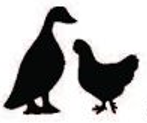
\includegraphics[scale=0.2]{artikel/poultry}      & (G)     & Contains poultry (usually chicken).                                \\
        \hline
        \rule{0pt}{1cm+1ex}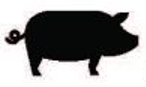
\includegraphics[scale=0.2]{artikel/pork}         & (S)     & Contains pork.                                                     \\
        \hline
        \rule{0pt}{1cm+1ex}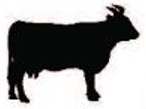
\includegraphics[scale=0.2]{artikel/beef}         & (R)     & Contains beef.                                                     \\
        \hline
        \rule{0pt}{1cm+1ex}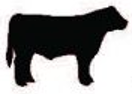
\includegraphics[scale=0.2]{artikel/veal}         & (K)     & Contains veal (meat from calves).                                  \\
        \hline
        \rule{0pt}{1cm+1ex}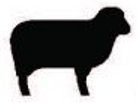
\includegraphics[scale=0.2]{artikel/lamb-mutton}  & (L)     & Contains lamb or mutton.                                           \\
        \hline
        \rule{0pt}{1cm+1ex}
\includegraphics[scale=0.2]{artikel/venison-game} & (W)     & Contains venison or other game meat.                               \\
        \hline
        \rule{0pt}{1cm+1ex}
\includegraphics[scale=0.2]{artikel/fish}         & (F)     & Contains fish.                                                     \\
        \hline
    \end{tabular}

    \begin{multicols}{2}
}{Johannes Alef, edited by Stefan Gries}
